\chapter{Respostas}
\pagestyle{plain}
\footnotesize

\pagecolor{gray!40}

\colorsec{Módulo 1 – Treino}

	\begin{enumerate}

	\item

	SAEB: Compor ou decompor números racionais positivos (representação
decimal finita) na forma aditiva, ou em suas ordens, ou em adições e
multiplicações.

BNCC: EF06MA01 -- Comparar, ordenar, ler e escrever números naturais e
números racionais cuja representação decimal é finita, fazendo uso da
reta numérica.

Alternativa A: incorreta, pois o aluno pode ter uma mal interpretação e
contar as classes ao invés das ordens.

Alternativa B: incorreta, pois o aluno pode ter uma mal interpretação e
considerar que as ordens são um conjunto de 3 números após o ponto.

Alternativa C: correta, pois são 4 ordens ao total.

Alternativa D: incorreta, pois o aluno pode compreender que ordens são a
soma de todos os números descritos.

	\item

	SAEB: Converter uma representação de um número racional positivo para
outra representação.

BNCC: EF06MA05 -- Classificar números naturais em primos e compostos,
estabelecer relações entre números, expressas pelos termos ``é múltiplo
de'', ``é divisor de'', ``é fator de'', e estabelecer, por meio de
investigações, critérios de divisibilidade por 2, 3, 4, 5, 6, 8, 9, 10,
100 e 1000.

Alternativa A: incorreta, o aluno pode esquecer de somar um ``X''.

Alternativa B: correta, pois essa é a representação em numerais romanos.

Alternativa C: incorreta, o aluno pode compreender que IX é 11 ao invés
de 9.

Alternativa D: incorreta, o aluno pode esquecer de somar a idade do
irmão mais novo.

	\item

	SAEB: Converter uma representação de um número racional positivo para
outra representação.

BNCC: EF06MA01 -- Comparar, ordenar, ler e escrever números naturais e
números racionais cuja representação decimal é finita, fazendo uso da
reta numérica.

Alternativa A: incorreta, pois o aluno pode considerar que a letra ``D''
representa ``Dezena'', logo o valor seria esse.

Alternativa B: correta, pois essa é a representação dos números.

Alternativa C: incorreta, pois o aluno pode confundir e contar um ``I''
a mais e considerar que o valor correto é esse.

Alternativa D: incorreta, pois o aluno pode considerar que a letra D
signifique Duzentos, logo o resultado seria esse.

	\end{enumerate}

\colorsec{Módulo 2 – Treino}

	\begin{enumerate}

		\item SAEB: Resolver problemas que envolvam as ideias de múltiplo, divisor,
máximo divisor comum ou mínimo múltiplo comum.

BNCC: EF06MA06 -- Resolver e elaborar problemas que envolvam as ideias
de múltiplo e de divisor.

Alternativa A: incorreta, pois o aluno pode realizar a somar a soma ao
invés de calcular o m.m.c.

Alternativa B: incorreta, pois o aluno pode considerar que o valor do
m.m.c. em si já é a resposta.

Alternativa C: incorreta, pois o aluno pode confundir m.m.c. com m.d.c.
nos cálculos e chegar a esse resultado.

Alternativa D: correta, pois somando o resultado do m.m.c. com o ano de
1984 obtemos este valor.

		\item SAEB: Resolver problemas que envolvam as ideias de múltiplo, divisor,
máximo divisor comum ou mínimo múltiplo comum.

BNCC: EF06MA07 -- Compreender, comparar e ordenar frações associadas às
ideias de partes de inteiros e resultado de divisão, identificando
frações equivalentes.

Alternativa A: incorreta, pois O aluno pode confundir o resultado do
m.d.c. dos valores como resposta.

Alternativa B: incorreta, pois o aluno pode calcular incorretamente o
m.d.c. esquecendo do valor 5 no final, onde o resultado seria esse.

Alternativa C: incorreta, pois o aluno pode esquecer de contar um número
``2'' no cálculo do m.d.c.

Alternativa D: correta, pois, calculando o m.d.c., obtemos 24,
realizando a operação 1080: 24 obtemos 45.

		\item SAEB: Resolver problemas que envolvam as ideias de múltiplo, divisor,
máximo divisor comum ou mínimo múltiplo comum.

BNCC: EF06MA06 -- Resolver e elaborar problemas que envolvam as ideias
de múltiplo e de divisor.

Alternativa A: incorreta, pois o aluno pode considerar correta essa
alternativa caso ele considere que se encontram no mesmo dia de todo
mês.

Alternativa B: incorreta, pois o aluno pode chegar a esse resultado se
considerar que outubro tenha 30 dias.

Alternativa C: correta, pois realizando o m.m.c., temos 42 dias. 20 dias
depois de 20 de setembro cairá no dia 1 de novembro, lembrando que
outubro tem 31 dias.

Alternativa D: incorreta, pois o aluno pode considerar que setembro
tenha 31 dias.

	\end{enumerate}

\colorsec{Módulo 3 – Treino}

	\begin{enumerate}

		\item SAEB: Representar frações menores ou maiores que a unidade por meio de
representações pictóricas ou associar frações a representações
pictóricas.

BNCC: EF06MA09 -- Resolver e elaborar problemas que envolvam o cálculo
da fração de uma quantidade e cujo resultado seja um número natural, com
e sem uso de calculadora.

Alternativa A: incorreta, pois o aluno provavelmente efetuou a operação
de maneira incorreta.

Alternativa B: correta, pois 2/4 = (2 x 2) / (4 x 2) = 4/8
\textgreater{} 3/8; logo, Maria comeu mais torta.

Alternativa C: incorreta, pois a operação demonstra que Maria e João
comeram porções diferentes.

Alternativa D: incorreta, pois o aluno deve saber comparar frações
diferentes.

		\item SAEB: Identificar frações equivalentes.

BNCC: EF06MA09 -- Resolver e elaborar problemas que envolvam o cálculo
da fração de uma quantidade e cujo resultado seja um número natural, com
e sem uso de calculadora.

Alternativa A: correta, pois:

Para comparar frações elas devem possuir os denominadores iguais. Para
isso, calculamos o MMC entre 5, 4, 3 e 9, que são os denominadores das
frações sorteadas.

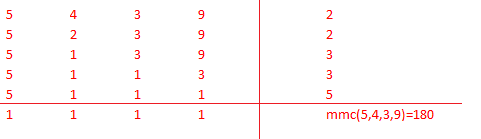
\includegraphics[width=5.01042in,height=1.44792in]{./imgSAEB_6_MAT/media/image36.png}

Para encontrar as frações equivalentes, dividimos 180 pelos
denominadores das frações sorteadas e, multiplicamos o resultado pelos
numeradores.

Para 3/5

180 / 5 = 36, como 36 x 3 = 108, a fração equivalente será 108 / 180.

Para 1/4

180/4 = 45, como 45 x 1 = 45, a fração equivalente será 45/180

Para 2/3

180/3 = 60, como 60 x 2 = 120, a fração equivalente será 120/180

Para 5/9

180/9 = 20, como 20 x 5 = 100. A fração equivalente será 100/180

Com as frações equivalentes, basta ordenar pelos numeradores em ordem
crescente e associar com as frações sorteadas. Logo 1/4, 5/9, 3/5, 2/3.

Alternativa B: incorreta, O aluno pode considerar que quanto maior o
denominador, maior o valor fracionário, assim 1/4 seria uma fração maior
que 2/3.

Alternativa C: incorreta, o aluno pode se confundir na forma de calcular
o m.m.c. e colocar erroneamente as frações de forma incorreta.

Alternativa D: incorreta, o aluno pode se confundir e colocar as frações
em forma decrescente ao invés de crescente.

		\item SAEB: Representar frações menores ou maiores que a unidade por meio de
representações pictóricas ou associar frações a representações
pictóricas

BNCC: EF06MA09 -- Resolver e elaborar problemas que envolvam o cálculo
da fração de uma quantidade e cujo resultado seja um número natural, com
e sem uso de calculadora.

Alternativa A: incorreta, pois o aluno pode erroneamente considerar que
ambos os potes de sorvete foram divididos em 3 partes.

Alternativa B: incorreta, pois o aluno erroneamente pode considerar que
somando as partes de chocolates de ambos os potes sem calcular o m.m.c.
pode se tornar uma resposta correta.

Alternativa C: correta, pois: o primeiro pote continha 3 sabores em
iguais quantidades: 1/3 de chocolate, 1/3 de baunilha e 1/3 de morango.
No segundo pote, havia 1/2 de chocolate e 1/2 de baunilha. Considerando
os dois potes de sorvete, dividimos os dois potes em partes iguais.
Fazendo então o m.m.c. de (2,3), obtemos que cada pote foi dividido em 6
partes iguais. Portanto nos dois potes temos 12 partes iguais. Sendo que
destas, 5 partes correspondem ao sabor chocolate.

Alternativa D: incorreta, o aluno pode considerar dividir os potes em 3
partes iguais e somar sem calcular o m.m.c., que chegará a esse
resultado erroneamente.

	\end{enumerate}

\colorsec{Módulo 4 – Treino}

	\begin{enumerate}

		\item SAEB: Resolver problemas que envolvam porcentagens, incluindo os que
lidam com acréscimos e decréscimos simples, aplicação de percentuais
sucessivos e determinação de taxas percentuais.

BNCC: EF06MA13 -- Resolver e elaborar problemas que envolvam
porcentagens, com base na ideia de proporcionalidade, sem fazer uso da
``regra de três'', utilizando estratégias pessoais, cálculo mental e
calculadora, em contextos de educação financeira, entre outros.

Alternativa A: incorreta, pois o aluno pode considerar que aumentar 25\%
signifique aumentar 25 centavos.

Alternativa B: incorreta, pois o aluno pode calcular erroneamente 1,20 x
0,025, chegando a esse resultado equivocado.

Alternativa C: incorreta, poiso aluno pode considerar que 25\% tenha
relação com o valor R\$1,25, pela semelhança.

Alternativa D: correta, pois R\$ 1,20 x 0,25 = 0,3, logo somando R\$1,20
+ R\$0,30 temos 1,50

		\item SAEB: Resolver problemas que envolvam porcentagens, incluindo os que
lidam com acréscimos e decréscimos simples, aplicação de percentuais
sucessivos e determinação de taxas percentuais.

BNCC: EF06MA13 -- Resolver e elaborar problemas que envolvam
porcentagens, com base na ideia de proporcionalidade, sem fazer uso da
``regra de três'', utilizando estratégias pessoais, cálculo mental e
calculadora, em contextos de educação financeira, entre outros.

Alternativa A: incorreta, pois aluno pode deduzir que ao multiplicar o
valor por 0,68 que o valor logo terá 68 \% de desconto.

Alternativa B: incorreta, pois o aluno pode deduzir que, ao multiplicar
o valor por 0,68, os livros terão 6,8 \% devido à semelhança dos termos.

Alternativa C: incorreta, pois o cálculo pode ser feito corretamente mas
a semelhança de 3,2\% para 32\% pode confundir o aluno na hora de
decisão de assinalar a resposta correta.

Alternativa D: correta, pois, ao multiplicar qualquer valor de livro por
68\%, obtém-se um desconto de 32\%.

		\item SAEB: Resolver problemas que envolvam porcentagens, incluindo os que
lidam com acréscimos e decréscimos simples, aplicação de percentuais
sucessivos e determinação de taxas percentuais.

BNCC: EF06MA13 -- Resolver e elaborar problemas que envolvam
porcentagens, com base na ideia de proporcionalidade, sem fazer uso da
``regra de três'', utilizando estratégias pessoais, cálculo mental e
calculadora, em contextos de educação financeira, entre outros.

Alternativa A: incorreta, pois o aluno pode realizar o cálculo
corretamente, mas confundir os valores próximos de R\$1.555, 00 com
R\$1.545, 00 devido à semelhança.

Alternativa B: incorreta, pois o aluno, por meio de dedução, pode
considerar que, somando 3\% ao valor inicial e subtraindo 3\%, o valor
inicial fique inerte.

Alternativa C: correta, pois:

Cálculo do acréscimo

1500 · 0,03 = 45

1.550 + 45 = 1.545

Cálculo do desconto

1.545 · 0,03 = 46,35

1.545 - 46,35 = 1.498,65

Alternativa D: incorreta, pois o aluno, por meio de dedução, pode
considerar que, somando 3\% ao valor inicial e subtraindo 3\%, o valor
inicial fique inerte.
	
	\end{enumerate}

\colorsec{Módulo 5 – Treino}

	\begin{enumerate}

		\item SAEB: Resolver problemas que possam ser representados por sistema de
equações de 1º grau com duas incógnitas.

BNCC: EF06MA14 -- Reconhecer que a relação de igualdade matemática não
se altera ao adicionar, subtrair, multiplicar ou dividir os seus dois
membros por um mesmo número e utilizar essa noção para determinar
valores desconhecidos na resolução de problemas.

Alternativa A: incorreta, pois o aluno pode chegar à conclusão de que o
número de bolas vermelhas é 72, dividindo por 4 ao tentar encontrar o
número de bolas amarelas.

Alternativa B: incorreta, pois o aluno pode considerar que o enunciado
pede o número de bolas amarelas.

Alternativa C: incorreta, pois o aluno pode realizar a operação 360:4,
obtendo um resultado incorreto.

Alternativa D: correta, pois, realizando o sistema, temos que:

X + Y = 360

X = 4y

Inserindo o valor de X na primeira equação, temos que:

4y + y = 360

5y = 360

y = 72

Realizando 360 - 72 = 288, temos o valor correto de bolas vermelhas.

		\item SAEB: Resolver problemas que possam ser representados por sistema de
equações de 1º grau com duas incógnitas.

BNCC: EF06MA14 -- Reconhecer que a relação de igualdade matemática não
se altera ao adicionar, subtrair, multiplicar ou dividir os seus dois
membros por um mesmo número e utilizar essa noção para determinar
valores desconhecidos na resolução de problemas.

Alternativa A: incorreta, pois o aluno durante a resolução pode
confundir e ao invés de dividir 8 por 0,05, realizar a multiplicação.

Alternativa B: incorreta, pois o aluno pode resolver a equação
erroneamente, calculando 0,05 : 8.

Alternativa C: correta, pois, ao substituir t por 8, temos:

8 = 0,05 . x

8/0,05 = x

x = 160

Alternativa D: incorreta, pois o aluno pode erroneamente colocar o valor
8 na incógnita x.

		\item SAEB: Resolver problemas que possam ser representados por sistema de
equações de 1º grau com duas incógnitas.

BNCC: EF06MA14 -- Reconhecer que a relação de igualdade matemática não
se altera ao adicionar, subtrair, multiplicar ou dividir os seus dois
membros por um mesmo número e utilizar essa noção para determinar
valores desconhecidos na resolução de problemas.

Alternativa A: correta, pois, considerando:

x = quantidade do produto A em gramas

y = quantidade do produto B em gramas

x + y = 100 (I)

x·A + y·B = 3,60 (II)

De (I), deduzimos:

y = 100 - x

Que aplicamos em (II):

x·A + (100-x)·B = 3,60

Substituindo A e B pelos seus custos em reais:

x·0,03 + (100-x)y·0,05 = 3,60

Multiplicando toda a equação acima por 100, a fim de tornar inteiros
seus coeficientes:

x·3 + (100-x)·5 = 360

3x + 500 - 5x = 360

-2x = 360 - 500

-2x = -140

x = -140/-2

x = 70 gramas

Alternativa B: incorreta, pois o aluno pode simplesmente retirar a
quantidade de gramas do enunciado e considerar como resposta correta.

Alternativa C: incorreta, pois o aluno pode considerar o preço final do
produto como resposta correta.

Alternativa D: incorreta, pois o aluno pode esquecer de dividir a
equação final por 2, chegando a esse resultado.

	\end{enumerate}

\colorsec{Módulo 6 – Treino}

	\begin{enumerate}

		\item SAEB: Resolver problemas que envolvam variação de proporcionalidade
direta ou inversa entre duas ou mais grandezas, inclusive escalas,
divisões proporcionais e taxa de variação.

Alternativa A: correta, pois, ao realizar a regra de 3 simples, obtemos
o valor de 2 máquinas.

Alternativa B: incorreta, pois o aluno pode esquecer de realizar a
conversão de uma hora para meia hora, chegando a esse resultado
erroneamente.

Alternativa C: incorreta, pois o aluno pode, ao invés de realizar o
cruzamento na regra de três, multiplicar linearmente, chegando a esse
resultado.

Alternativa D: O aluno pode realizar a conversão corretamente, mas errar
o cruzamento no cálculo de regra de três, chegando a esse valor
erroneamente.

		\item SAEB: Resolver problemas que envolvam variação de proporcionalidade
direta ou inversa entre duas ou mais grandezas, inclusive escalas,
divisões proporcionais e taxa de variação.

Alternativa A: incorreta, pois o aluno pode realizar o cruzamento de
dados erroneamente na regra de 3 e chegar a esse valor.

Alternativa B: correta, pois, realizando a regra de 3 composta, obtemos
o valor 35.

Alternativa C: incorreta, pois, ao esquecer que as apostilas não tem
mais 27 folhas e sim 35, o aluno chega a esse resultado erroneamente.

Alternativa D: incorreta, pois, caso o aluno esqueça de ler todo o
enunciado, ele não compreenderá que os minutos de funcionamento da
impressora 2 diminuem, chegando a essa resposta.

		\item SAEB: Resolver problemas que envolvam variação de proporcionalidade
direta ou inversa entre duas ou mais grandezas, inclusive escalas,
divisões proporcionais e taxa de variação.

Alternativa A: incorreta, pois, caso o aluno realize a multiplicação da
regra de 3 sem cruzamentos, chegará a esse valor.

Alternativa B: incorreta, pois, ao calcular o cruzamento da regra de 3
erroneamente, o alunochegará a esse valor.

Alternativa C: incorreta, pois, ao confundir o resultado em horas com
minutos, o aluno acabará assinalando essa alternativa erroneamente.

Alternativa D: correta, pois realizando a regra de três composta,
obtemos esse valor.

	\end{enumerate}

\colorsec{Módulo 7 – Treino}

	\begin{enumerate}

		\item SAEB: Resolver problemas que envolvam relações entre os elementos de uma
circunferência/círculo (raio, diâmetro, corda, arco, ângulo central,
ângulo inscrito).

BNCC: EF06MA18 -- Reconhecer, nomear e comparar polígonos, considerando
lados, vértices e ângulos, e classificá-los em regulares e não
regulares, tanto em suas representações no plano como em faces de
poliedros.

Alternativa A: incorreta, pois o aluno pode esquecer que o valor do raio
é a metade do diâmetro, chegando nesse valor.

Alternativa B: incorreta, pois ao confundir a fórmula do perímetro da
circunferência com a fórmula da área da circunferência chegará a esse
valor.

Alternativa C: incorreta, pois, ao realizar uma soma ao invés de uma
multiplicação na fórmula, obterá esse valor.

Alternativa D: correta, pois ao considerar pi = 3, temos que 2.3.6 =
36cm

		\item SAEB: Resolver problemas que envolvam relações entre os elementos de uma
circunferência/círculo (raio, diâmetro, corda, arco, ângulo central,
ângulo inscrito).

BNCC: EF06MA18 -- Reconhecer, nomear e comparar polígonos, considerando
lados, vértices e ângulos, e classificá-los em regulares e não
regulares, tanto em suas representações no plano como em faces de
poliedros.

Alternativa A: correta, pois, ao calcular a fórmula da área do círculo,
temos que A= 3 . 10² = 300m²

Alternativa B: incorreta, pois, ao realizar o cálculo de perímetro da
circunferência, ao invés do cálculo da área chegaremos a esse valor.

Alternativa C: incorreta, pois o aluno pode esquecer de trocar o
diâmetro pelo raio na fórmula e chegará a esse valor.

Alternativa D: incorreta, pois o aluno pode esquecer de verificar que o
valor do enunciado se trata de m² e não cm².

		\item SAEB: Relacionar o número de vértices, faces ou arestas de prismas ou
pirâmides, em função do seu polígono da base.

BNCC: EF06MA17 -- Quantificar e estabelecer relações entre o número de
vértices, faces e arestas de prismas e pirâmides, em função do seu
polígono da base, para resolver problemas e desenvolver a percepção
espacial.

Alternativa A: correta, pois

V + F = A + 2

8 + 6 = A + 2

14 = A + 2

A = 14 - 2

A = 12 arestas

Alternativa B: incorreta, pois o aluno pode somar todos os números do
poliedro e chegar a essa conclusão equivocada.

Alternativa C: incorreta pois o aluno pode realizar uma subtração ao
invés de utilizar a fórmula.

Alternativa D: incorreta o aluno pode realizar uma multiplicação ao
invés de utilizar a fórmula.

	\end{enumerate}

\colorsec{Módulo 8 – Treino}

	\begin{enumerate}

		\item SAEB: Identificar relações entre ângulos formados por retas paralelas
cortadas por uma transversal.

BNCC: EF06MA19 -- Identificar características dos triângulos e
classificá-los em relação às medidas dos lados e dos ângulos.

Alternativa A: incorreta, pois o aluno pode chegar a essa conclusão
somando os valores literais e dividindo em seguida pelos números
restantes.

Alternativa B: incorreta, pois o aluno pode considerar multiplicar os
valores e dividir após o resultado para chegar a esse valor.

Alternativa c: correta, pois, Utilizando os conhecimentos sobre
bissetriz obtemos que as medidas dos Ângulos BÔP e PÔA são iguais, logo

2x+8=3x-10

2x-3x= -10 - 8

-x = -18

x = 18

Alternativa d: incorreta, pois o aluno, pela falta de conhecimento sobre
bissetriz, pode relembrar que 45 seja o valor da bissetriz do ângulo
reto e chegar a essa conclusão mesmo não se tratando de um ângulo reto.

		\item SAEB: Identificar relações entre ângulos formados por retas paralelas
cortadas por uma transversal.

BNCC: EF06MA19 -- Identificar características dos triângulos e
classificá-los em relação às medidas dos lados e dos ângulos.

Alternativa A: incorreta, pois o aluno errou na soma dos ângulos.

Alternativa B: incorreta, pois o aluno não soube aplicar a soma dos
ângulos internos.

Alternativa C: incorreta, pois o aluno não somou 80º para encontrar o
resultado correto.

Alternativa D: correta, pois a soma dos ângulos internos de um triângulo
é sempre igual a 180 graus. Se um dos ângulos mede 90 graus, a soma dos
outros dois ângulos deve ser igual a 180 - 90 = 90 graus.

		\item SAEB: Identificar relações entre ângulos formados por retas paralelas
cortadas por uma transversal.

BNCC: EF06MA19 -- Identificar características dos triângulos e
classificá-los em relação às medidas dos lados e dos ângulos.

Alternativa A: incorreta, pois o aluno pode considerar cortar mais peças
em relação àquilo que o enunciado recomenda.

Alternativa B: incorreta, pois o aluno pode considerar cortar mais peças
em relação àquilo que o enunciado recomenda.

Alternativa C: correta, pois, para cortar apenas 2 peças de madeira, o
brinquedo deverá ser um triangulo de lado 50 cm. Como será um triangulo
equilátero, terá 3 lados iguais.

Alternativa D: incorreta, pois o aluno pode considerar cortar mais peças
em relação àquilo que o enunciado recomenda.

	\end{enumerate}

\colorsec{Módulo 9 – Treino}

	\begin{enumerate}

		\item SAEB: Descrever ou esboçar deslocamento de pessoas e/ou de objetos em
representações bidimensionais (mapas, croquis etc.), plantas de
ambientes ou vistas, de acordo com condições dadas

BNCC: EF06MA21 -- Construir figuras planas semelhantes em situações de
ampliação e de redução, com o uso de malhas quadriculadas, plano
cartesiano ou tecnologias digitais.

Alternativa A: incorreta, pois o aluno pode esquecer de somar um
quadrinho e chegar a esse número.

Alternativa B: correta: pois, é utilizada a rota 20 + 10 + 30 + 20 + 10
= 90.

Alternativa C: incorreta, pois o aluno pode considerar seguir por uma
rota que não seja a mais vantajosa.

Alternativa D: incorreta, pois o aluno pode considerar seguir por uma
rota que não seja a mais vantajosa.

		\item 
SAEB: Descrever ou esboçar deslocamento de pessoas e/ou de objetos em
representações bidimensionais (mapas, croquis etc.), plantas de
ambientes ou vistas, de acordo com condições dadas

BNCC: EF06MA21 -- Construir figuras planas semelhantes em situações de
ampliação e de redução, com o uso de malhas quadriculadas, plano
cartesiano ou tecnologias digitais.

Alternativa A: correta, pois as coordenadas indicam essa localização.

Alternativa B: incorreta, pois o aluno pode se perder na condução do
mapa e chegar a essa conclusão erroneamente.

Alternativa C: incorreta, pois o aluno pode se perder na condução do
mapa e chegar a essa conclusão erroneamente.

Alternativa D: incorreta, pois o aluno pode se perder na condução do
mapa e chegar a essa conclusão erroneamente.

		\item SAEB: Descrever ou esboçar deslocamento de pessoas e/ou de objetos em
representações bidimensionais (mapas, croquis etc.), plantas de
ambientes ou vistas, de acordo com condições dadas

BNCC: EF06MA21 -- Construir figuras planas semelhantes em situações de
ampliação e de redução, com o uso de malhas quadriculadas, plano
cartesiano ou tecnologias digitais.

Alternativa A: correta, pois essa definição está correta.

Alternativa B: incorreta, pois as primeiras definições estão incorretas.

Alternativa C: incorreta, pois a definição de planta está incorreta.

Alternativa D: incorreta, pois há diferenças entre esses conceitos.

	\end{enumerate}
\colorsec{Módulo 10 – Treino}

\colorsec{Módulo 11 – Treino}

\colorsec{Módulo 12 – Treino}